\documentclass[conference]{IEEEtran}
\usepackage{cite}
\usepackage{amsmath,amssymb,amsfonts}
\usepackage{algorithm}
\usepackage{algorithmic}
\usepackage{graphicx}
\usepackage{textcomp}
\usepackage{xcolor}
\usepackage{multicol}
\usepackage{float}
\usepackage[spanish]{babel}

\def\BibTeX{{\rm B\kern-.05em{\sc i\kern-.025em b}\kern-.08em
    T\kern-.1667em\lower.7ex\hbox{E}\kern-.125emX}}
\begin{document}

\title{Esteganografía en Imágenes}
\author{\IEEEauthorblockN{Joaquín Pérez Araya}
\IEEEauthorblockA{\textit{Departamento de Ciencias de la Computación} \\
\textit{Universidad de Chile}\\
Santiago, Chile \\
joaquin.perez.a@ug.uchile.cl}}


\maketitle

\begin{abstract}
    Dentro del presente documento se tratará la Esteganografía en imágenes, un método de ocultación de mensajes en imágenes, tambien se discutirá el diseño e implementación de un programa que codifica mensajes utilizando los canales de la imagen, finalmente se realizan experimentos utilizando una imagen pequeña y otra grande, junto con textos pequeños y largos, para observar y determinar la cantidad de bits posibles que se pueden utilizar para codificar los mensajes sin perder la calidad visual de la imagen y el rendimiento que se tiene al codificar.
\end{abstract}
 

\section*{Introducción} % ***Así la cosa no me molesta con los numeritos***
    A lo largo de la historia de la humanidad ha existido la necesidad de envíar información ocultos, ya sea para transmitir información sensible, como estrategias militares, mensajes de amor o incluso mera diversión.
    Uno de los modos es a través de la Esteganografía, que se diferencia de la Criptografía donde los mensajes son visibles pero inentendibles, por lo que la Esteganografía se dedica a ocultar mensajes desapercibidamente al ojo humano.
    Dado por el contexto del curso, se considerarán sólo Esteganografía sobre imágenes, hay variados métodos, con niveles de seguridad variados, desde escribir después del indicador \texttt{EOF} el mensaje a esconder \cite{DIS}, el que fue implementado, hasta utilizar el histograma de la imagen para guardar el contenido del mensaje.
    En este documento se enfocará sobre una implementación de Esteganografía sobre imagenes, que consiste en codificar los caracteres de un texto a una imagen utilizando uno de sus canales.
    
\section*{Diseño e Implementación}
	Para la implementación del programa se utilizó Python 3.6 con las librerías \texttt{numpy}, \texttt{sci-kit-image} y \texttt{argparse}. El código está dividido en 4 partes: Utilidades, Entrada/Salida, Codificación y Decodificación.
\subsection*{Entrada y Salida}
    Para el uso externo del programa por medio de comandos se utilizó la librería \texttt{argparse} que viene por defecto en Python. Leer los comandos dados y traducirlos a llamados directos a las funciones de codificación o decodificación, tal como se pide en los requisitos de la tarea.
    	
	\subsection*{Utilidades}
	El módulo de utilidades (\texttt{util.py}) están las funciones auxiliares que utilizan la codificación y decodificación entre las de las cuales se destacan:
	\begin{itemize}
	    \item \texttt{image\_read}\footnotemark, \texttt{image\_write} y \texttt{text\_read}: Son las funciones para leer los archivos externos que se van a utilizar para el proceso de codificación y decodificación.
         
	    \footnotetext{La función que está implementada en el código es la que está en \texttt{pai\_io.py} dentro del repositorio del curso.}
	    	    
        \item \texttt{text\_to\_ascii} y \texttt{ascii\_to\_text}: La primera se utiliza para codificar el mensaje mientras que la segunda para decodificar. Se usan para transformar una cadena de texto a una lista de números donde cada caracter es un número de la lista y viceversa.
        
        \item \texttt{to\_binary} y \texttt{to\_int}: Se utilizan para codificar y decodificar, ya que reduce el problema de inserción de bits a modificar las cadenas de texto en binario\footnote{Con cadena de texto binaria se refiere a una cadena de texto que es la representación binaria de un número.} de los valores del canal de imagen.
        
        \item \texttt{join\_binaries}: Se usa modificar la cadena de texto binaria para codificar un caracter en éste, une dos cadenas de texto, reemplazando los últmos $n$ caracteres de la cadena por los $n$ caracteres del segundo. Retorna un entero.
        
        \item \texttt{last\_value}: Se utiliza para obtener los bits menos significativos de un número, para obtener el caracter que está codificado es éste.
	\end{itemize}
	
	\subsection*{Codificación}
        La codificación consta de una única función que dada la una dirección de imagen, una dirección texto y un número de bits $n$ realice todo el proceso de abrir la imagen, obtener el primer canal de información para modificarlo con la finaldiad de agregarle la información que corresponde al texto. \\
        
		Dado el texto a codificar, éste se convierte el texto a codificar a una lista de números\footnote{Usando \texttt{text\_to\_ascii}.} donde cada letra se le asigna un número que corresponde al valor en \texttt{ascii} del caracter, finalmente se agrega un último elemento $0$ para agregar un final de codificación para el decodificador.        
        Dado el primer canal de la imagen\footnote{Se usa el primero para evitar diferenciación al usar imagenes a color y en blanco y negro.}, se copia y en esta copia se codifica en los cuatros bits menos significativos del primer pixel ($0,0$) el número de bits que se van a usar en los siguientes para facilitar la acción de decodificación. Posteriormente, se utiliza la lista creada anteriormente para tomar los números de forma ordenada y traducirlos a binario, para insertarlos iterativamente. \\ 
        Por cada cadena de texto binaria se toma sus últimos $n$ bits y se insertan\footnote{Se insertan usando \texttt{join\_binaries}} hasta que la cadena de texto ya no se puede insertar complentamente, por lo que la ésta se inserta al final de la siguiente cadena binaria del siguiente carácter. Hasta agotar todos los caracteres de la lista.
    
        Dado a que cada símbolo en \texttt{ascii} es un número de 8 bits y en cada píxel se elige la cantidad de bits a codificar, éste método permite codificar $\lfloor (p-1)(bits / 8)\rfloor - 1$ caracteres como máximo dentro de una imagen con $p$ píxeles en total, ya que en el primer pixel de la imagen siempre se va a utilizar para guardar la cantidad de bits utilizado en los 4 bits menos significativos de éste, tambien se necesita codificar un caracter adicional para indicar que no se debe seguir decodificando. De forma inversa dado $c$ caracteres se necesitan $\lceil (c+1)(8 / bits)\rceil +1 $ pixeles.

	\subsection*{Decodificación}
		La decodficación sólo necesita la imagen para decodificar. Se extrae el primer canal de color, ya que durante la codificación se utilizó el primer pixel para codificar la cantidad de bits, se obtiene esta cantidad $n$ para proceder a rearmar los caracteres tomando los valores de los primeros $n$ bits en binario de los valores del canal de color hasta obtener 8 o más, para sacar los primeros 8 caracteres, transformalos en un número y agregarlos a la lista que se va a convertir en texto. El proceso se termina cuando se inserta en la lista el número $0$ o en su forma binaria \texttt{00000000}. 
		
		
\section*{Experimentación}
    Inicialmente para el testeo del funcionamiento inicial de la implementación se utilizó una imagen en negro de \texttt{10x10} pixeles con la finalidad de verificar vía simple inspección la codificación/decodificación. \\
    
\begin{figure}[H]
\begin{multicols}{3}
    \centering
    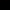
\includegraphics[width=0.95\linewidth]{image/black2.png} \par
    
\includegraphics[width=0.95\linewidth]{image/black4.png} \par
    
\includegraphics[width=0.95\linewidth]{image/black8.png} \par
\end{multicols}
\caption{El texto \texttt{Hola}, codificado usando 2, 4 y 8 bits para almacenar los datos (de izquierda a derecha).}
\end{figure}

	Es mucho más notable el rojo con una codificación con más bits que con menos, sin embargo el coste de codificar con menos bits es que se necesita una imagen más grande para poder agregar un mismo mensaje. Usando la fórmula obtenida anteriormente en el diseño de la codificación, obteniendo un gráfico que es con rendimientos decrecientes respecto a los bits.
	
\begin{figure}[H]
    \centering
    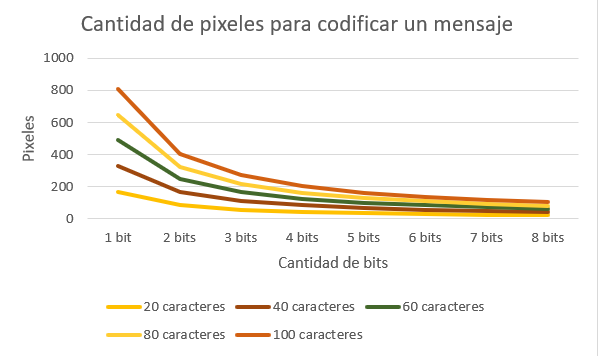
\includegraphics[width=0.95\linewidth]{image/Grafico2.png}
\caption{Gráfico que compara la cantidad de pixeles necesarios para codificar un mensaje con bits y cantidad de caracteres fijas.}
\end{figure}
	
	Por lo que no resulta tan beneficioso aumentar la cantidad de bits utilizados dentro de la imagen.
   
   Para experimentar en grande las diferencias entre las diferentes codificaciones, se procedió a codificar el libro Génesis de la Biblia en inglés (189.245 caracteres), en una imagen de un Ave de tamaño \texttt{1242x1279} (1.588.518 pixeles). Las imagenes resultantes están en el anexo, dado la necesidad de espacio visual necesario para distinguir las diferentes codificaciones. La calidad visual no se llega a percibir si se usan 3 o menos bits de codificación, sin embargo es altamente visible la modificación de 4 bits en adelante, de hecho corrobora el efecto decreciento que se muestra en el gráfico, debido a que la distorción del color es notoria en áreas similares de la foto.
   Las imagenes están disponibles junto con el texto en los archivos que vienen con este informe.

\section*{Conclusión}
    En la sección anterior se estableció el límite de bits para no comprometer el estado de la imagen, considerando tambien los rendimientos decrecientes de utilizar más bits, los bits recomendados para codificar de forma segura una imagen serían, 2 y 3. La diferencia entre codificar en un bit y en dos es imperceptible, así codificar en un sólo bit se convierte más en una operación el doble de ineficiente si se compara la cantidad de pixeles se que necesitan para codificar el mismo mensaje.  
    Una de las consideraciones adicionales que se pueden llevar acabo utilizando este método sería el de utilizar más canalaes de la imagen para amplificar la cantidad de texto que se puede codificar, si la imagen fuese en color, ésta cantidad aumentaría al triple.
    
\begin{thebibliography}{99}
\bibitem{DIS} Cheddad, A., Condell, J., Curran, K., \& Mc Kevitt, P. (2010). Digital image 
steganography: Survey and analysis of current methods. Signal Processing, 90(3), 727–752. 


\end{thebibliography}

\section*{Anexo}
    \begin{figure}[H]
    \centering
    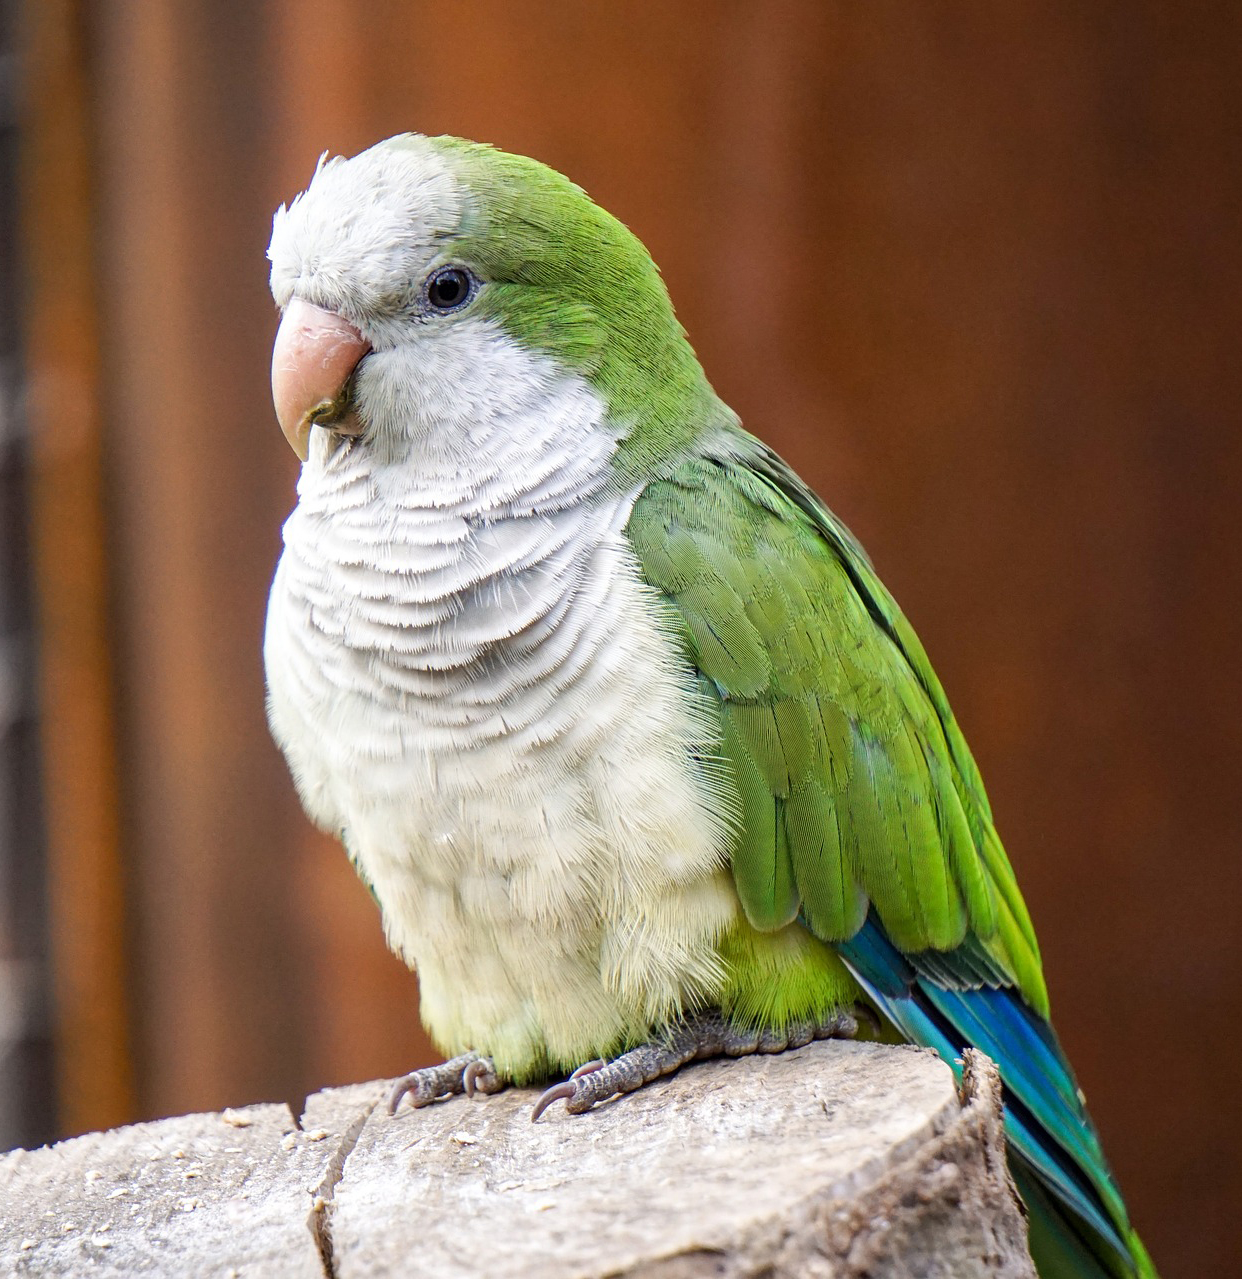
\includegraphics[width=0.9\linewidth]{image/birb.png}
\caption{Imagen de una Ave normal}
\end{figure}

    
    \begin{figure}[H]
    \centering
    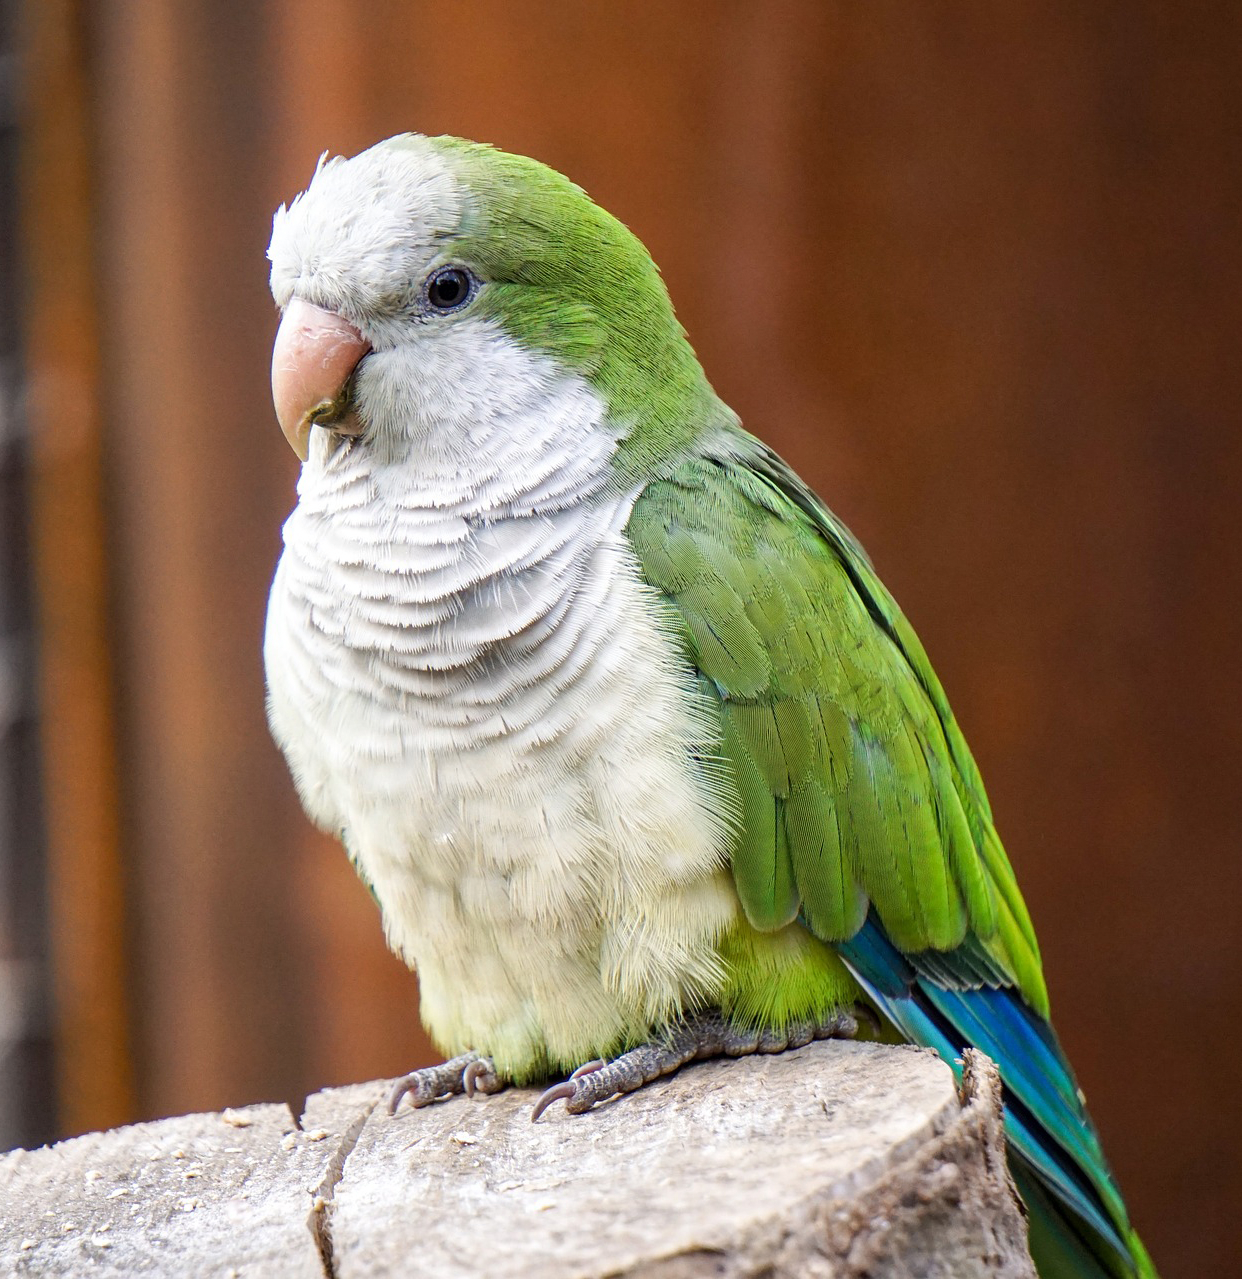
\includegraphics[width=0.9\linewidth]{image/birb1.png}
\caption{Imagen de una Ave, codificada con el Génesis en 1 bit.}
\end{figure}

    \begin{figure}[H]
    \centering
    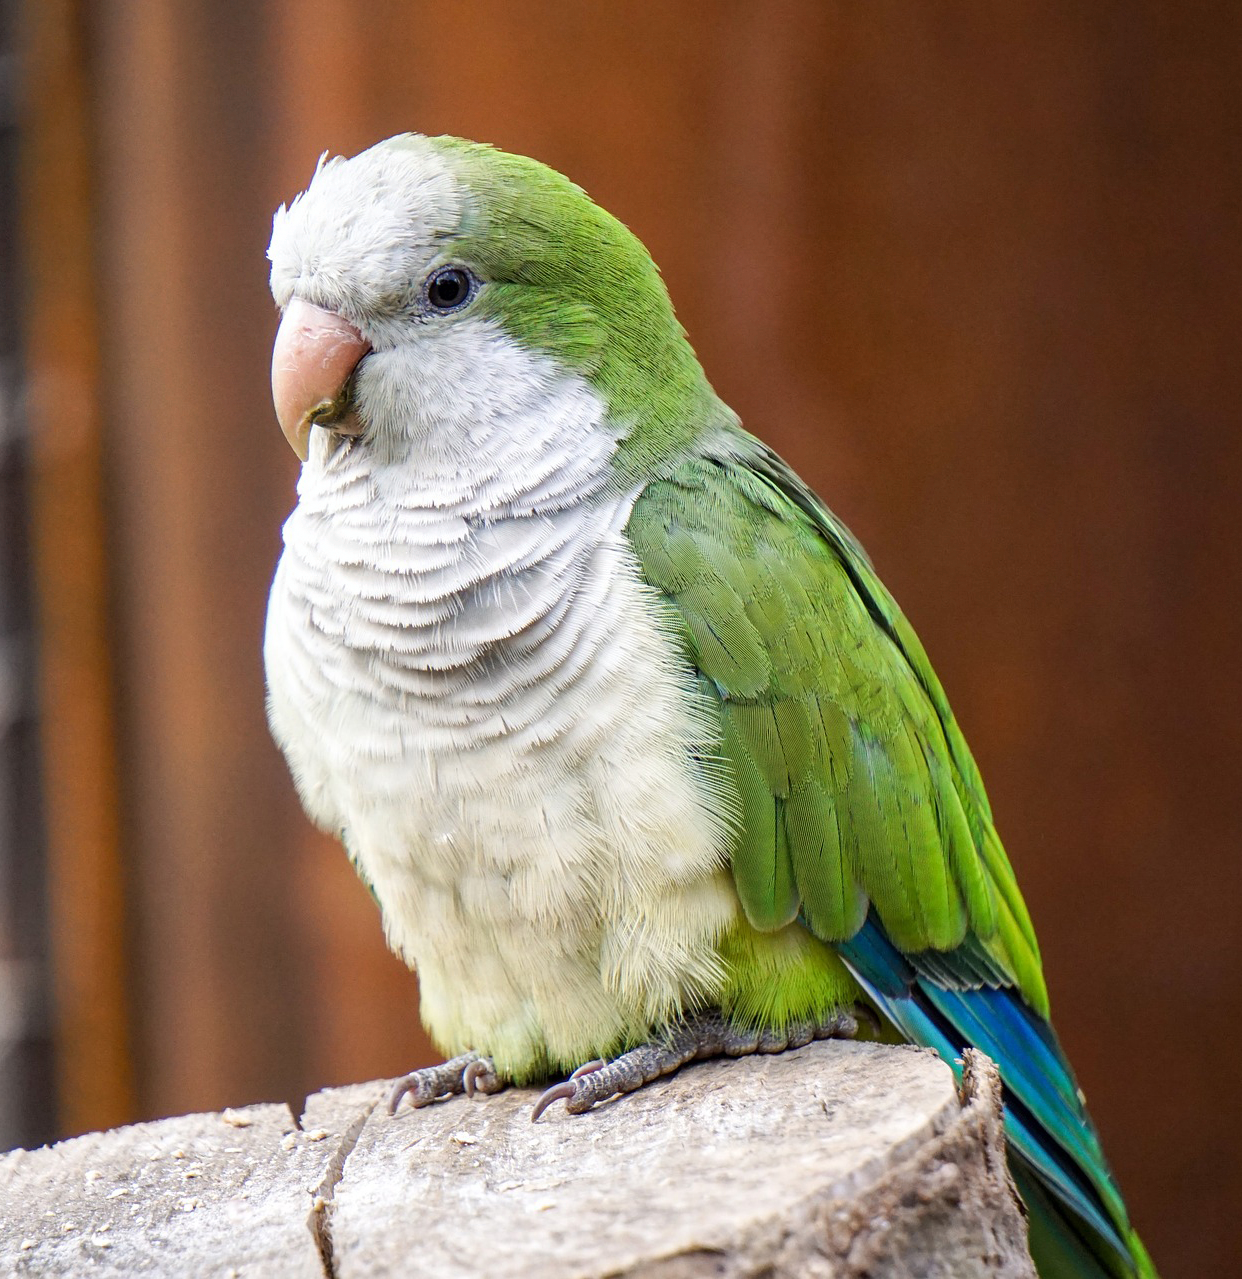
\includegraphics[width=0.9\linewidth]{image/birb2.png}
\caption{Imagen de una Ave, codificada con el Génesis en 2 bits.}
\end{figure}

    \begin{figure}[H]
    \centering
    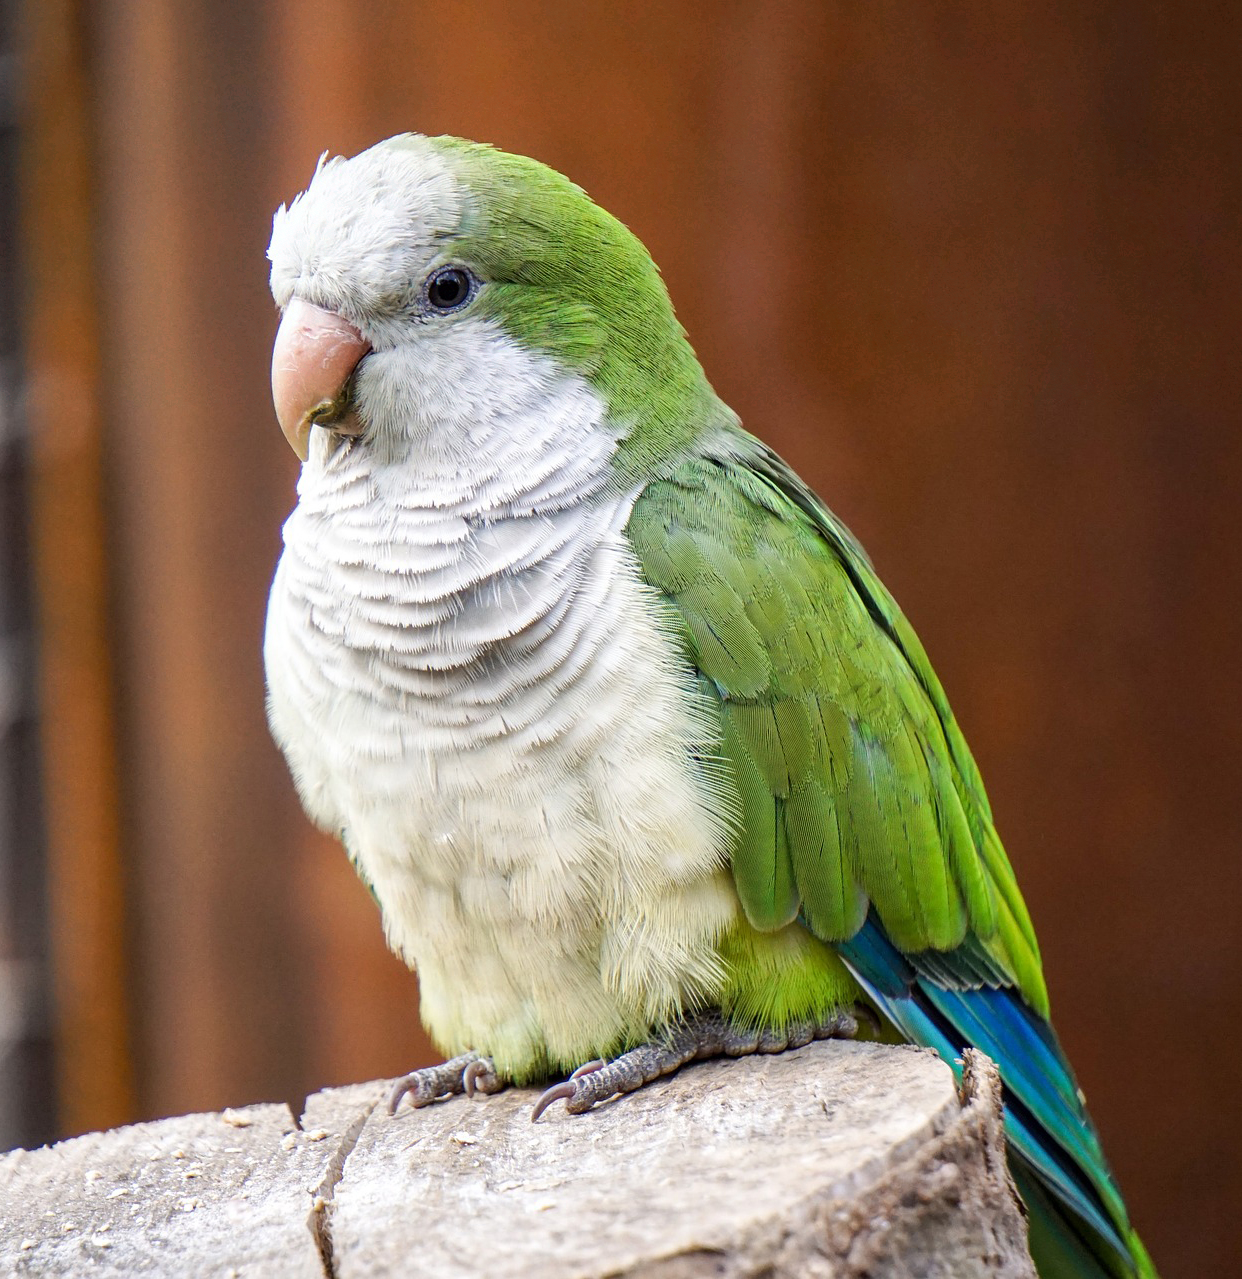
\includegraphics[width=0.9\linewidth]{image/birb3.png}
\caption{Imagen de una Ave, codificada con el Génesis en 3 bits.}
\end{figure}

    \begin{figure}[H]
    \centering
    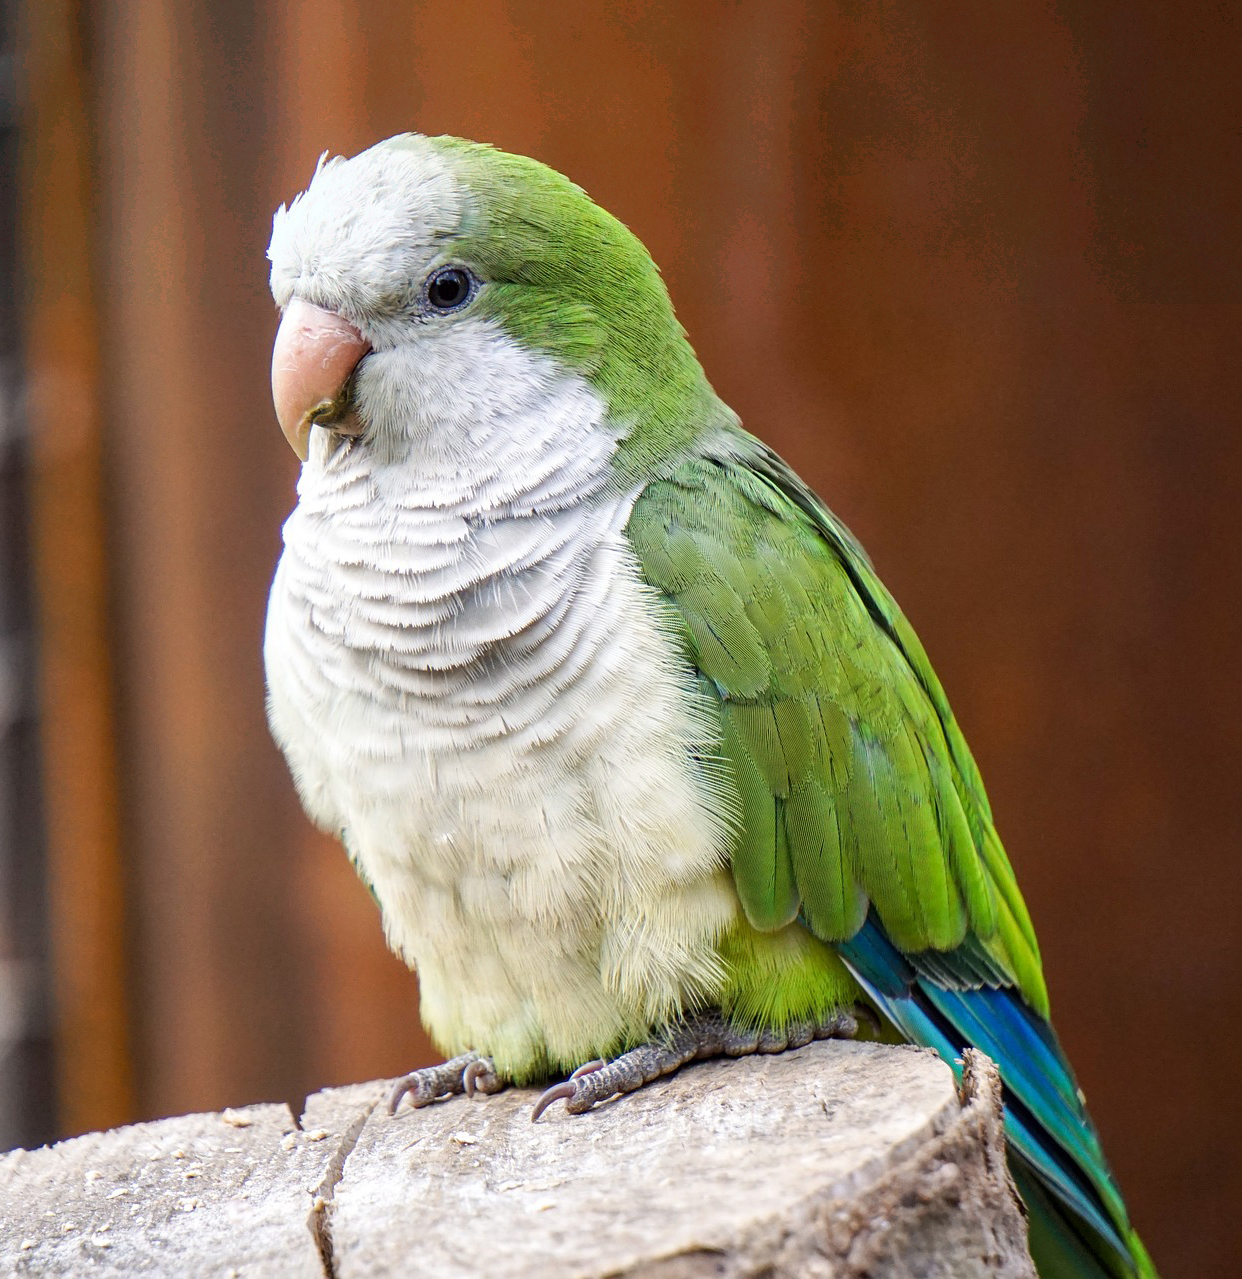
\includegraphics[width=0.9\linewidth]{image/birb4.png}
\caption{Imagen de una Ave, codificada con el Génesis en 4 bits.}
\end{figure}

    \begin{figure}[H]
    \centering
    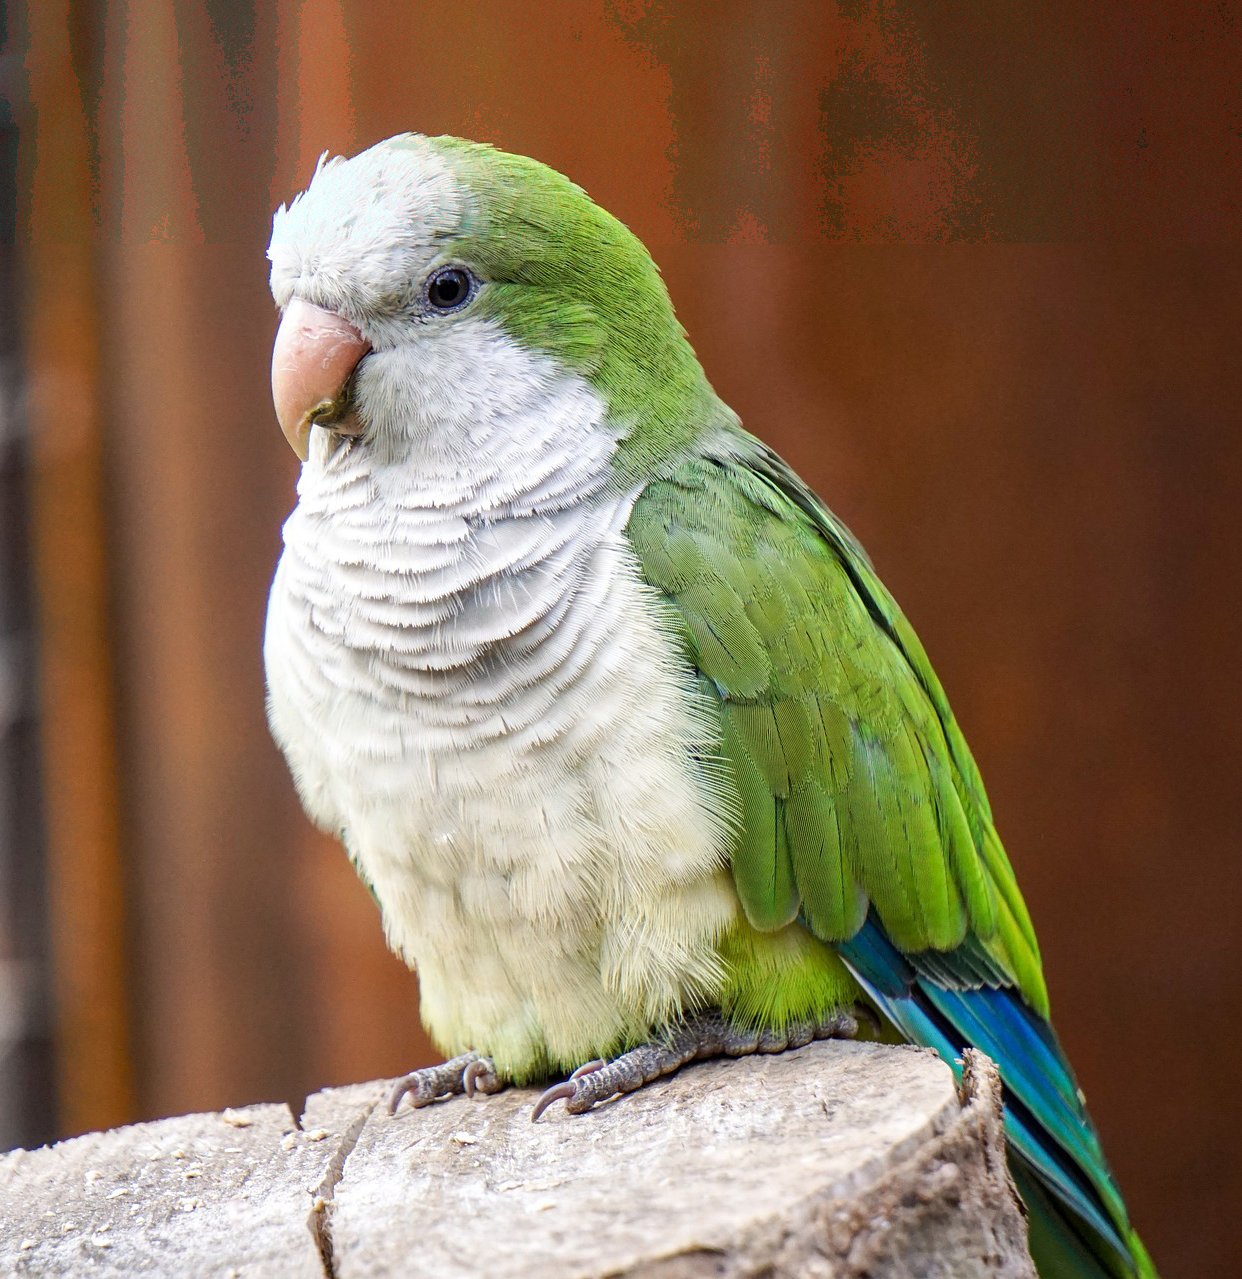
\includegraphics[width=0.9\linewidth]{image/birb5.png}
\caption{Imagen de una Ave, codificada con el Génesis en 5 bits.}
\end{figure}

    \begin{figure}[H]
    \centering
    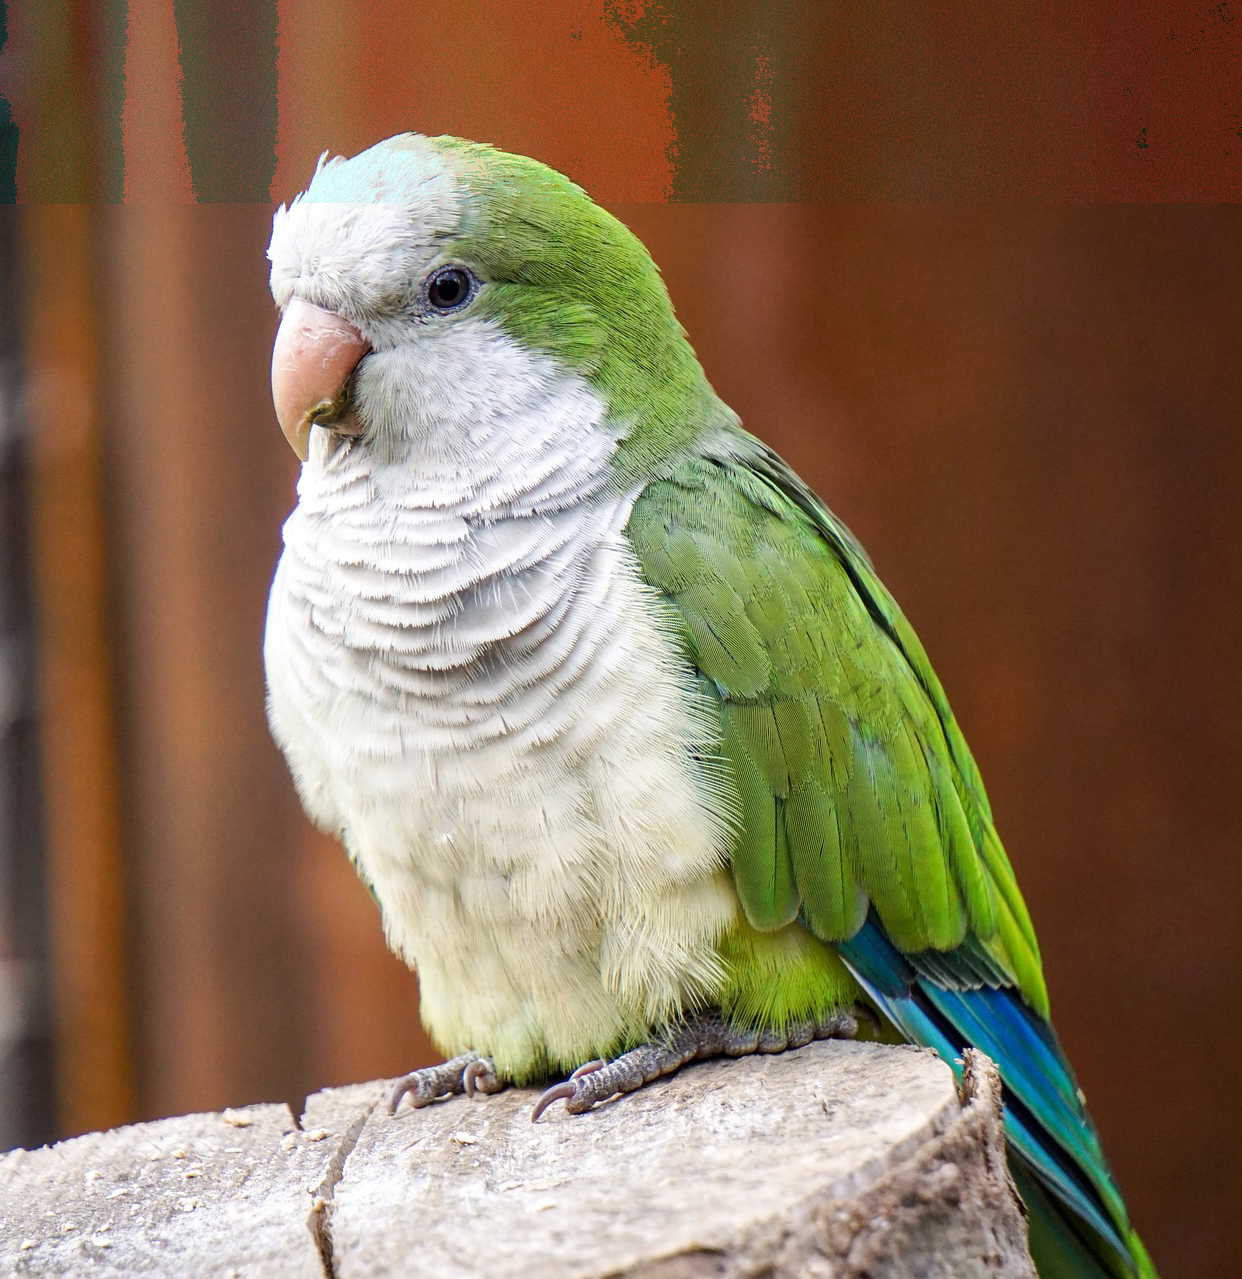
\includegraphics[width=0.9\linewidth]{image/birb6.png}
\caption{Imagen de una Ave, codificada con el Génesis en 6 bits.}
\end{figure}

    \begin{figure}[H]
    \centering
    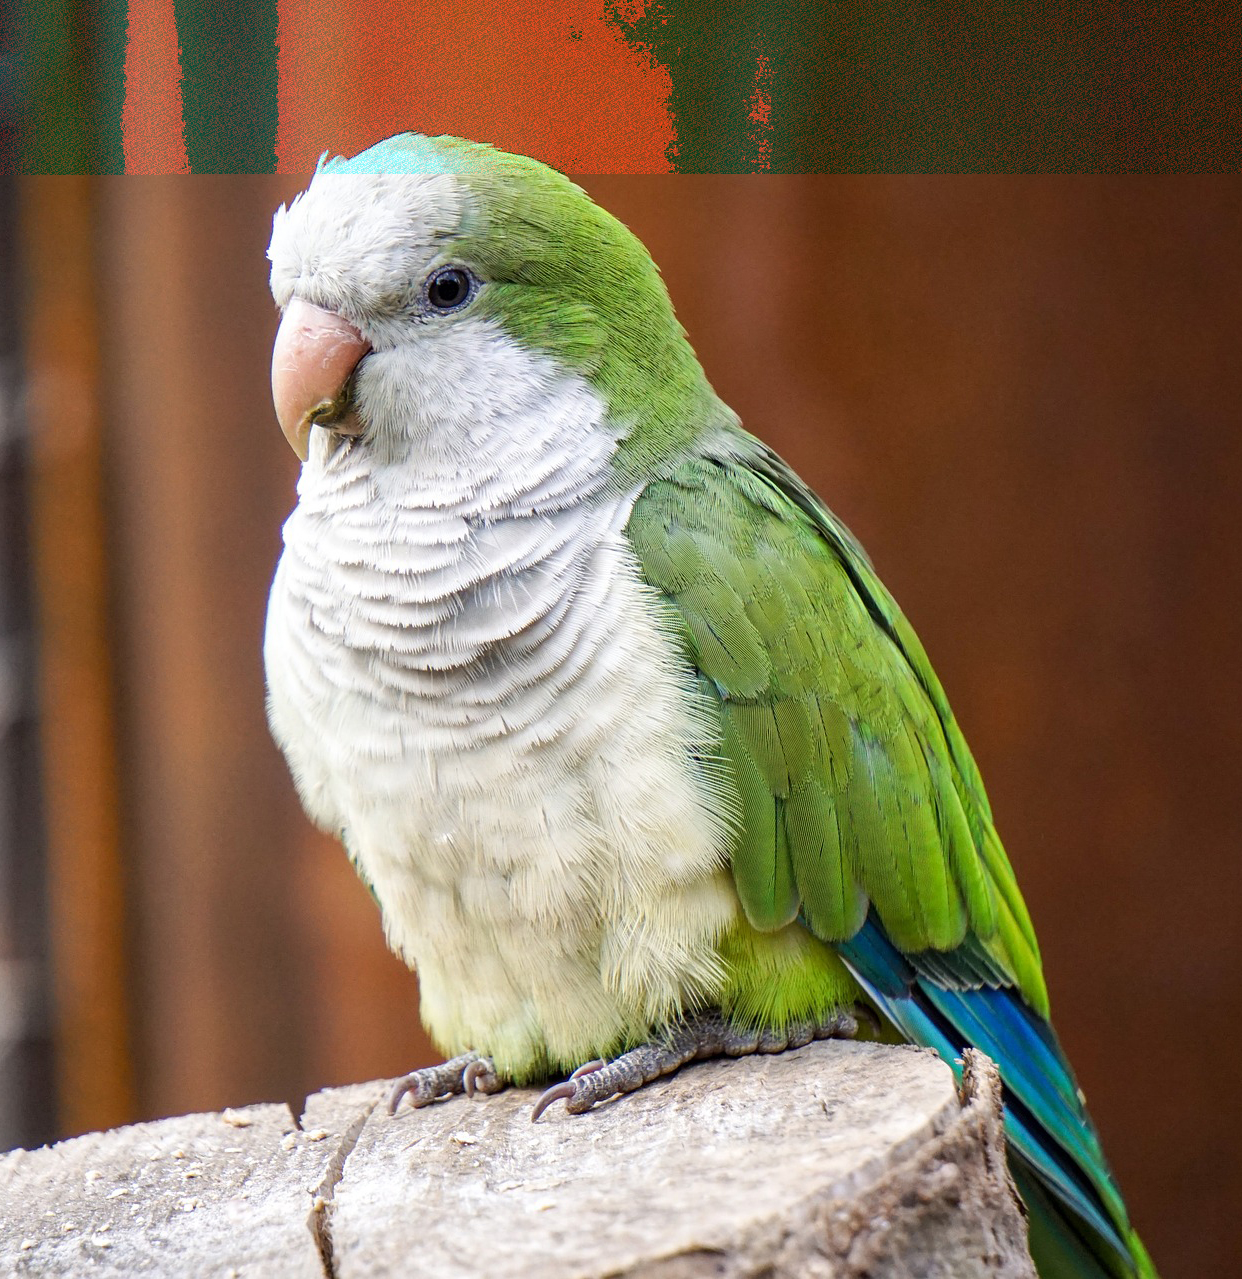
\includegraphics[width=0.9\linewidth]{image/birb7.png}
\caption{Imagen de una Ave, codificada con el Génesis en 7 bits.}
\end{figure}

    \begin{figure}[H]
    \centering
    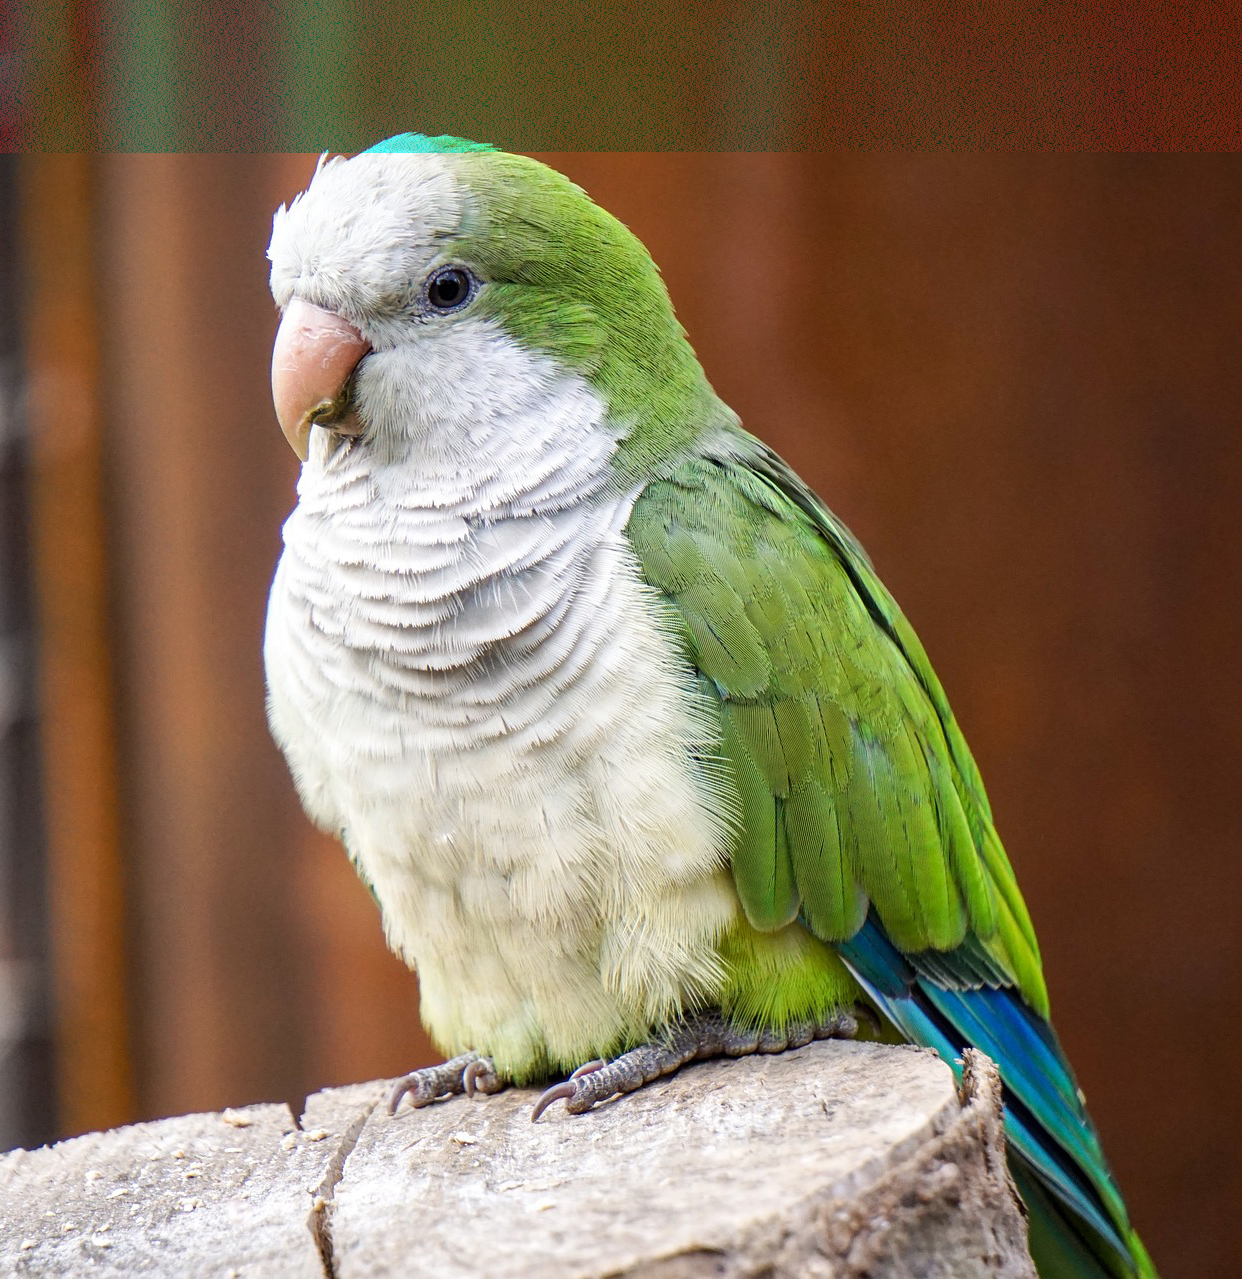
\includegraphics[width=0.9\linewidth]{image/birb8.png}
\caption{Imagen de una Ave, codificada con el Génesis en 8 bits}
\end{figure}
\end{document}
